\documentclass[a4paper, 10pt]{ctexart} %中文支持
\usepackage{float}              %防止浮动元素浮动
\usepackage{rotating}           %旋转图片用的
\usepackage{hyperref}           %用来生成一些可跳转的标签
\usepackage{amsfonts}           %对某一些字体之支持
\usepackage{amsmath}            %数学公式
\usepackage{amsthm}             %定义, 定理, 证明, 例子这些环境的支持
%使用方法:
%\newtheorem{environment name}{caption}
%比如 \newtheorem{example}{这是例子}
%效果 \begin{example} xxx \end{example} -> 这是例子 1 xxx
%proof就不需要了
\usepackage{graphicx}           %用来插入图片
\usepackage[left=1.25in,right=1.25in,top=1in,bottom=1in]{geometry}   %用来排版的
\usepackage[]{color}            %用来给部分文本上色的
\usepackage{algorithm}          %用来写伪代码的
\usepackage{algorithmic}        %同上
\usepackage{minted}
\usepackage{amssymb}            %用来加入一些数学符号, 比如说 $\varnothing$
\usepackage{fontspec}           %不知道用来干嘛的
%\setmonofont{Ubuntu Mono}       %?
%\usemintedstyle{custommanni}    %设置minted插入代码的风格
\usemintedstyle{vs}

\newtheorem{theorem}{定理}
\newtheorem{example}{Example}
\newtheorem{definition}{定义}
\newtheorem{lemma}{引理}
\title{算法作业第6章}
\author{毛翰翔 \and 210110531}
\date{\today}
\begin{document}
\maketitle
1、用本章知识解决下面的问题,写出你的思路和伪代码。

	在商店中, 有许多在售的物品。然而,也有一些大礼包,每个大礼包以优惠的价格捆绑销售一组物品。现给定每个物品的价格,每个大礼包包含物品的清单,以及待购物品清单。请输出确切完成待购清单的最低花费。每个大礼包由一个数组中的一组数据描述,最后一个数字代表大礼包的价格,其他数字分别表示内含的其他种类物品的数量。任意大礼包可无限次购买。

示例 1:

输入: [2,5], [[3,0,5],[1,2,10]], [3,2]

输出: 14


解释: 

有A和B两种物品,价格分别为¥2和¥5。


大礼包1,你可以以¥5的价格购买3A和0B。

大礼包2, 你可以以¥10的价格购买1A和2B。

你需要购买3个A和2个B, 所以你付了¥10购买了1A和2B(大礼包2),以及¥4购买2A。

示例 2:

输入: [2,3,4], [[1,1,0,4],[2,2,1,9]], [1,2,1]

输出: 11

解释: 

A,B,C的价格分别为¥2,¥3,¥4.

你可以用¥4购买1A和1B,也可以用¥9购买2A,2B和1C。

你需要买1A,2B和1C,所以你付了¥4买了1A和1B(大礼包1),以及¥3购买1B, ¥4购买1C。

你不可以购买超出待购清单的物品,尽管购买大礼包2更加便宜

说明:



	最多6种物品, 100种大礼包。
    
	每种物品,你最多只需要购买6个。
    
	你不可以购买超出待购清单的物品,即使更便宜。
    \\[7pt]
$\mathbf{Solution}$ : 基本思路是使用深度优先遍历. 使用递归函数. 

我们首先考察没有使用礼包的情况, 将其和使用了礼包的进行对比. 前者是能够求出的, 后者调用函数求出来. 

设这个函数是 \verb|dfs| , 假设使用了第 i 礼包, 那么对 needs 数组进行更新, 对于使用了礼包之后剩余的需求, 我们使用类似的方法, 先是考察不使用礼包的情况, 再考察使用了第 j 个礼包的情况. 

其中, i , j 都是任意的, 于是说每次递归调用都需要 Numof{}Special 次, 其中 Numof{}Special 是礼包的个数. 


\begin{minted}{c}
#define infty 100000
int dfs (int CurrentSpecial , int *ShinNeeds, int **special, int n, int *price, int NumofSpecial){
    int CopyNeeds[10] = {0};    // cpoy 一个数组, 向下进行一个传递. 
    int temp = 0, ans = 0;
    for (int i  = 0 ; i < n ; i++){
        CopyNeeds[i] = ShinNeeds[i] - special[CurrentSpecial][i];
                                // 根据这个礼包, 更新这个needs数组
        if (CopyNeeds[i] < 0)   // 如果说不用买这个礼包就直接返回最大值. 
        return infty;
    }
    // ans 更新为不买礼包的情况. 
    for (int i = 0 ; i < n ; i++)
        ans = ans + price[i] * CopyNeeds[i];
    // 遍历买各种礼包的情况.
    for (int i = 0 ; i < NumofSpecial ; i++){
        temp = dfs(i, CopyNeeds, special, n, price, NumofSpecial);
        if (temp < ans)
    // 如果说dfs结果更低一些, 就将ans更新.
            ans = temp;
    }
    return ans + special[CurrentSpecial][n];
}
int shoppingOffers(int* price, int priceSize, int** special, int specialSize, int* specialColSize, int* needs, int needsSize){
    int ans = infty;                // ans for answer
    int NumofSpecial = specialSize; // NumofSpecial , the number of specials
    int n = priceSize;              // n for number of items
    int temp; 
    for (int i = 0; i < NumofSpecial; i++){
        for (int j = 0; j < n+1; j++)
            scanf("%d", &special[i][j]);
    }
    // ans 更新为直接购入
    for (int i = 0; i < n; i++)
        ans = ans + needs[i] * price[i];
    // 
    for (int i = 0 ; i < NumofSpecial ; i++){
        temp = dfs(i , needs,special , n , price , NumofSpecial);
        if (temp < ans)
        ans = temp;
    }
    return ans;
}
\end{minted}

2. 给定一个4个点的连通有向图,其邻接矩阵如下:
\[\left[
\begin{matrix}
    \infty & 9 & 13 & 15 \\ 
    2 & \infty & 1 & 4 \\ 
    3 & 5 & \infty & 1 \\ 
    9 & 6 & 3 & \infty \\ 
\end{matrix}
\right]
\]
可用使用A*算法求这个图的旅行商问题。

(1)请写出你的g(n)和h*(n)的定义。

(2)画出求解此图的搜索树。
\\[7pt]
$\mathbf{solution}$: $g\left(n\right)$ 的定义是, 给定一个起点, 这个起点到 $n$ 的距离, $h^{*}\left(n\right)$ 的定义是, $n$ 经过剩下的顶点回到起点的最优值. 

类似的, 这里使用 ``连接了 $n$ 和未经过的节点的边'' 中最低权重. 作为 $h^{*}\left(n\right)$ 的一个下界.

这里我们使用 $1$ 为起点. 

\begin{figure}[H]
    \centering
    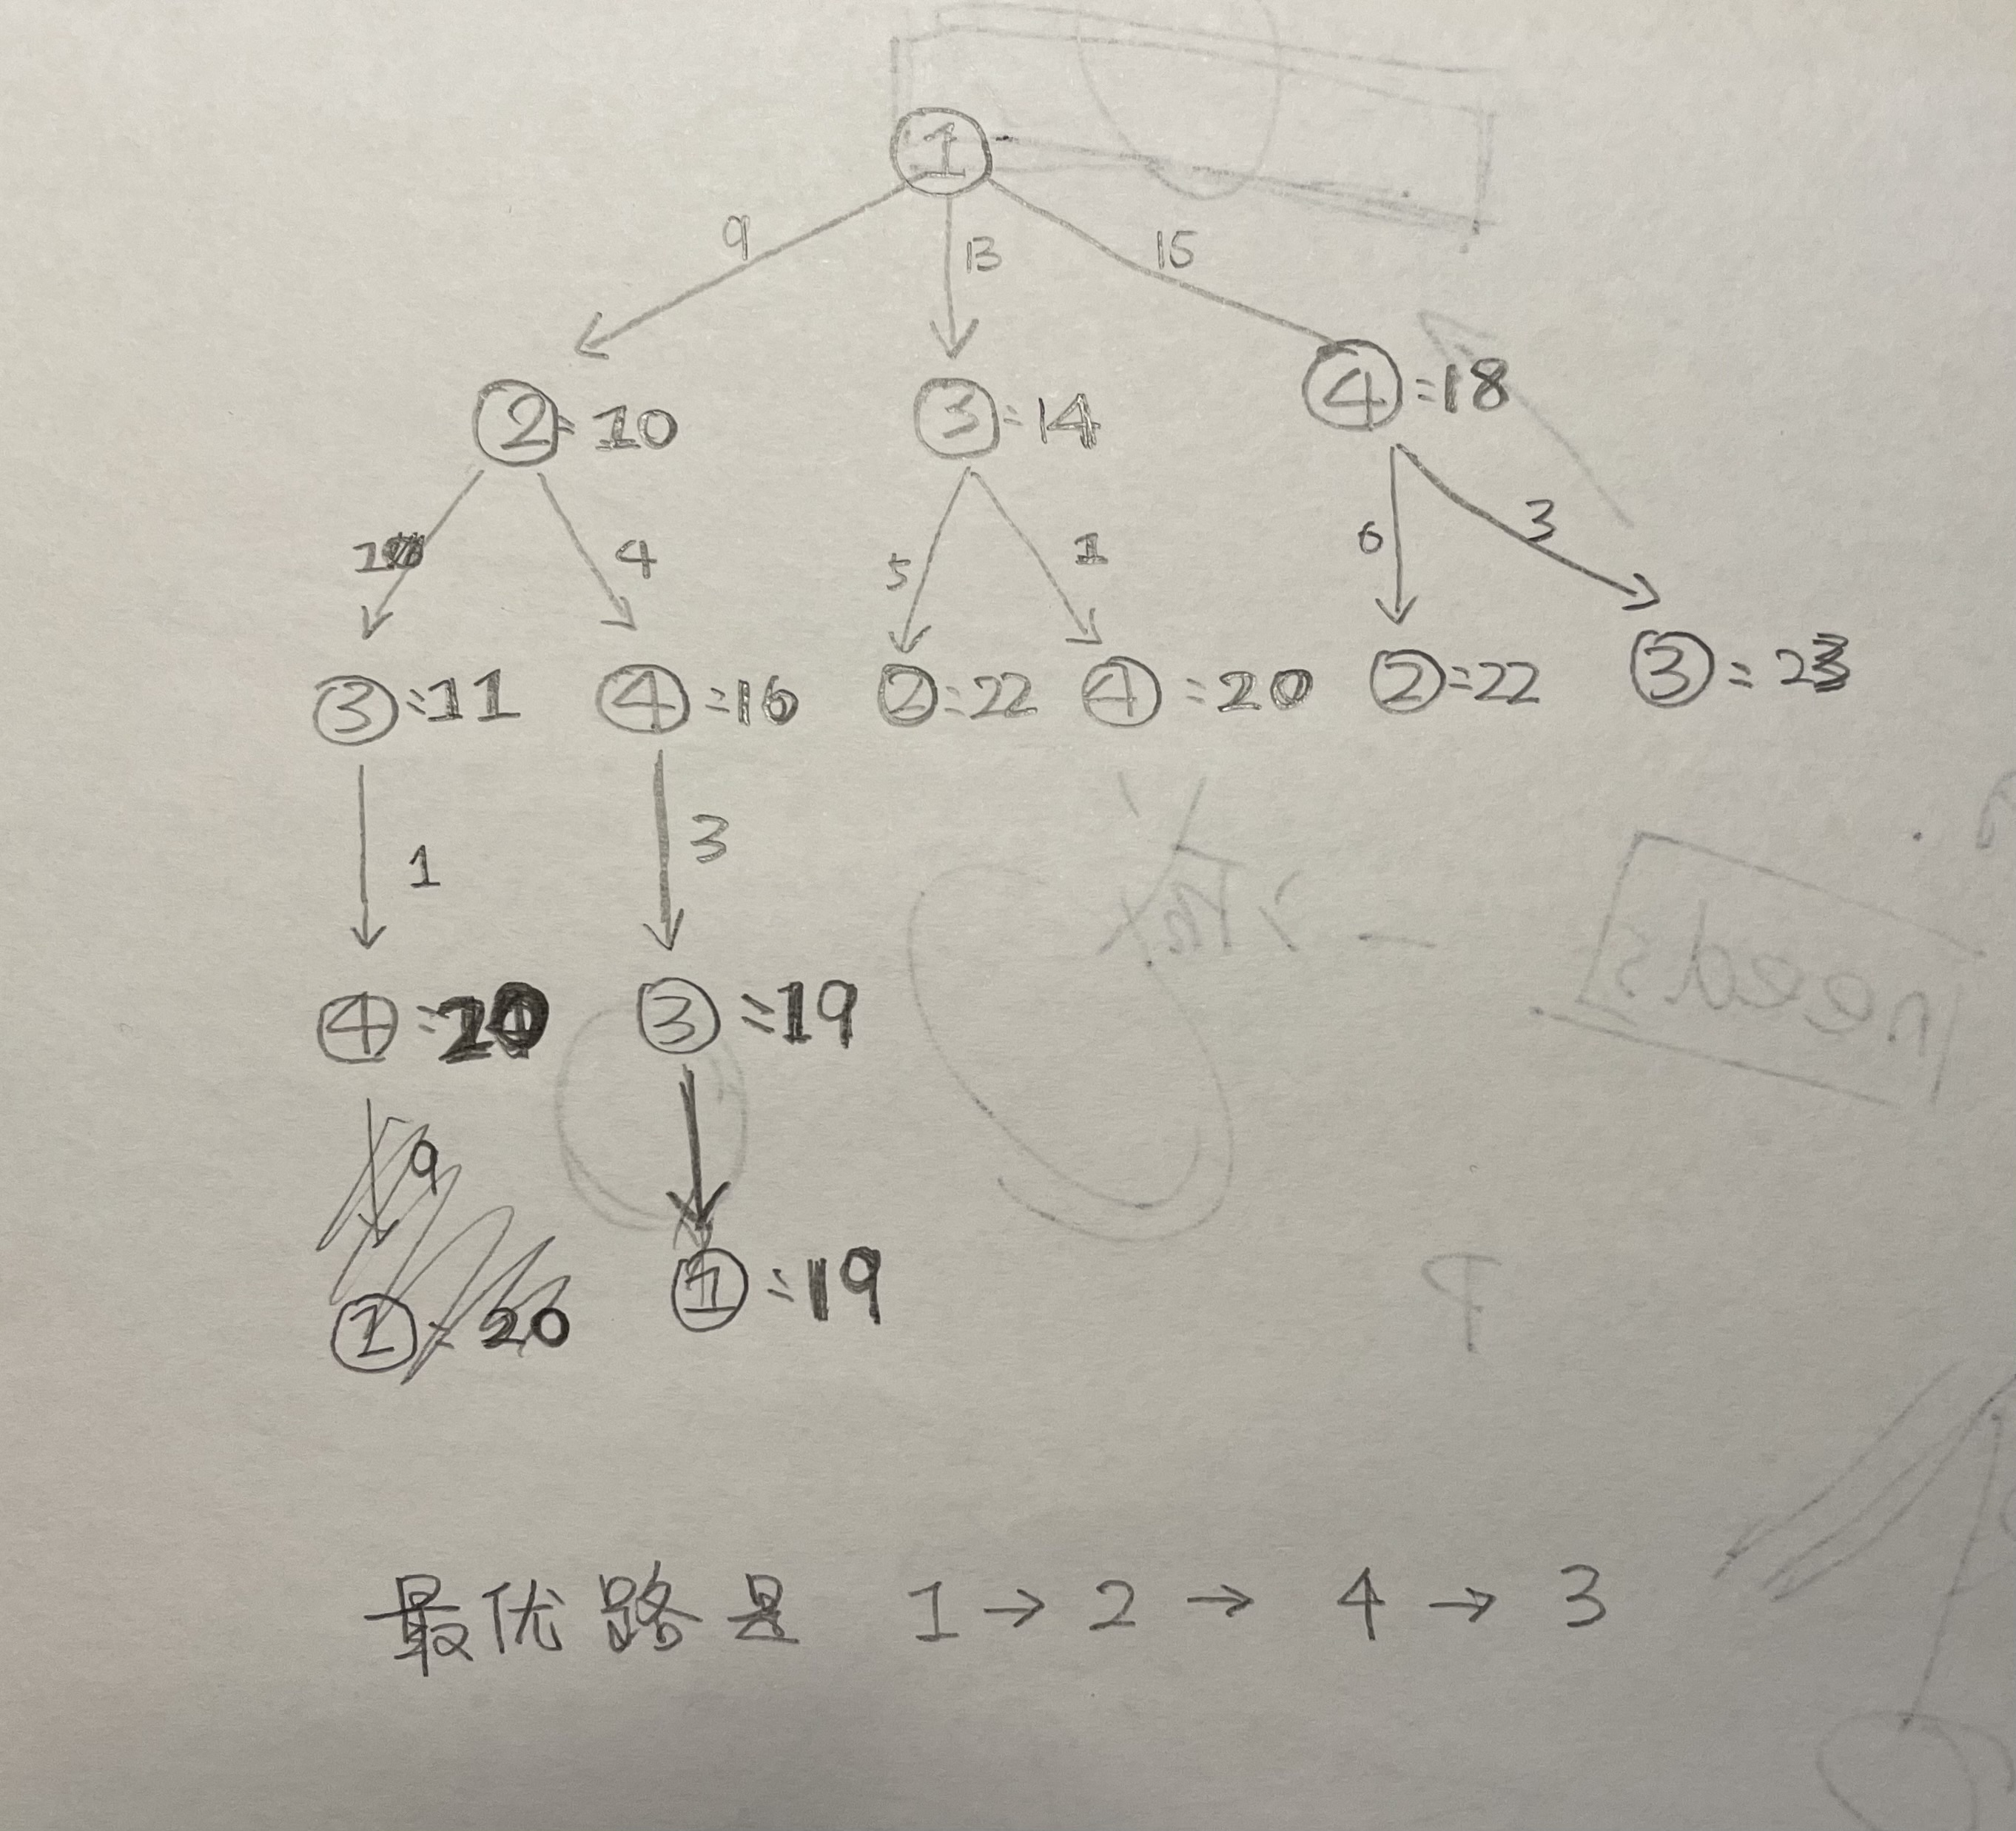
\includegraphics[scale = 0.5]{IMG_3053 1.jpg}
    \caption[]{树}
\end{figure}
\end{document}